\section{Speicher}
\vspace{-0.25cm}
\subsection{Speicherverbrauch}
\vspace{-0.25cm}
Ein essentieller Punkt in Bezug auf die maximal mögliche Baumtiefe in unserem Programm ist der Speicherverbrauch.
Maßgeblich ist hier das Array, in welchem die generierten Quader (Datentyp Cuboid) gespeichert werden. 
Die Größe eines Cuboids setzt sich wie folgt zusammen:
\vspace{0.25cm}\\
\begin{minipage}{0.4\linewidth}
    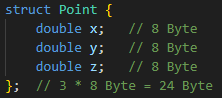
\includegraphics[width=\linewidth]{./pictures/SpeicherverbrauchPoint.PNG}
\end{minipage}
\hfill
\begin{minipage}{0.58\linewidth}
    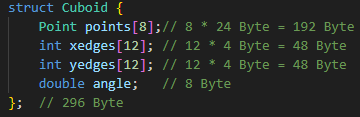
\includegraphics[width=\linewidth]{./pictures/SpeicherverbrauchCuboid.PNG}
\end{minipage}
\vspace{0.5cm}\\
Um die Daten sinnvoll im Speicher platzieren zu können, fügt der Compiler gegebenenfalls noch 8 Byte Padding pro Cuboid hinzu. 
Der Speicherplatzbedarf pro Quader liegt also bei 296 Byte oder 304 Byte. 
\vspace{0.5cm}\\
\begin{minipage}{0.55\linewidth}
    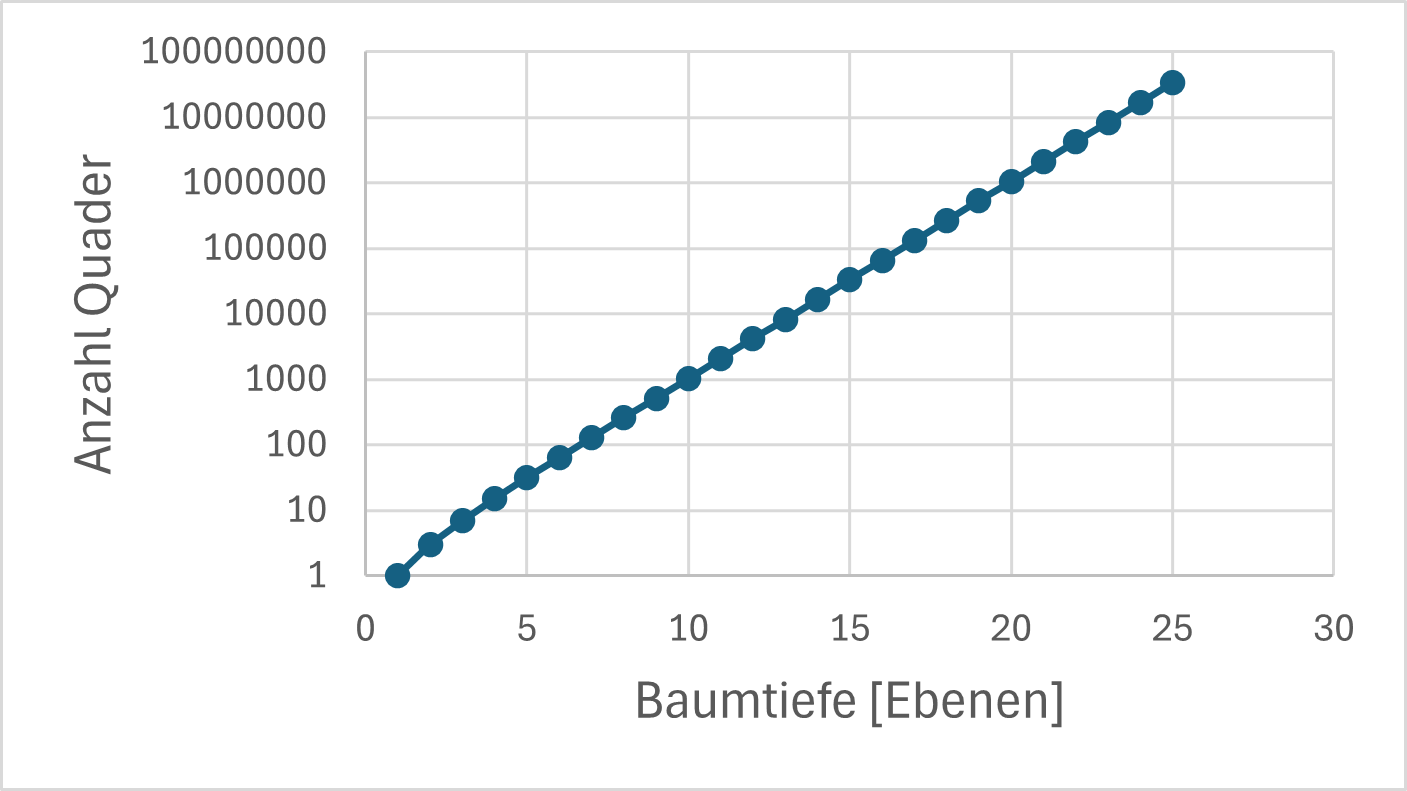
\includegraphics[width=\linewidth]{./diagrams/CuboidsProEbene.png}
    \captionof{figure}{Gesamtanzahl Quader pro Baumtiefe}
    \label{fig:CuboidsProEbene}
\end{minipage}
\hfill
\begin{minipage}{0.43\linewidth}
    Für jeden Quader in der aktuellen Ebene sind in der darauffolgenden Ebene zwei neue Quader zu generieren.
    Die Anzahl der zu generierenden Quader des Baums steigt also quadratisch mit der Funktion
    \vspace{-0.25cm} \center{$f(n) = 2^n - 1$,} \\
    wobei $n$ die Anzahl der Ebenen im Baum ist.
\end{minipage}
\vspace{0.5cm}

\noindent
\begin{minipage}{0.39\linewidth}
    Daraus ergibt sich, dass der benötigte Speicherplatz allein für die Quader ab einer Baumtiefe von 
21 Ebenen > 1 GB ist. Für 25 Ebenen werden annähernd 20 GB benötigt.
\end{minipage}
\hfill
\begin{minipage}{0.56\linewidth}
    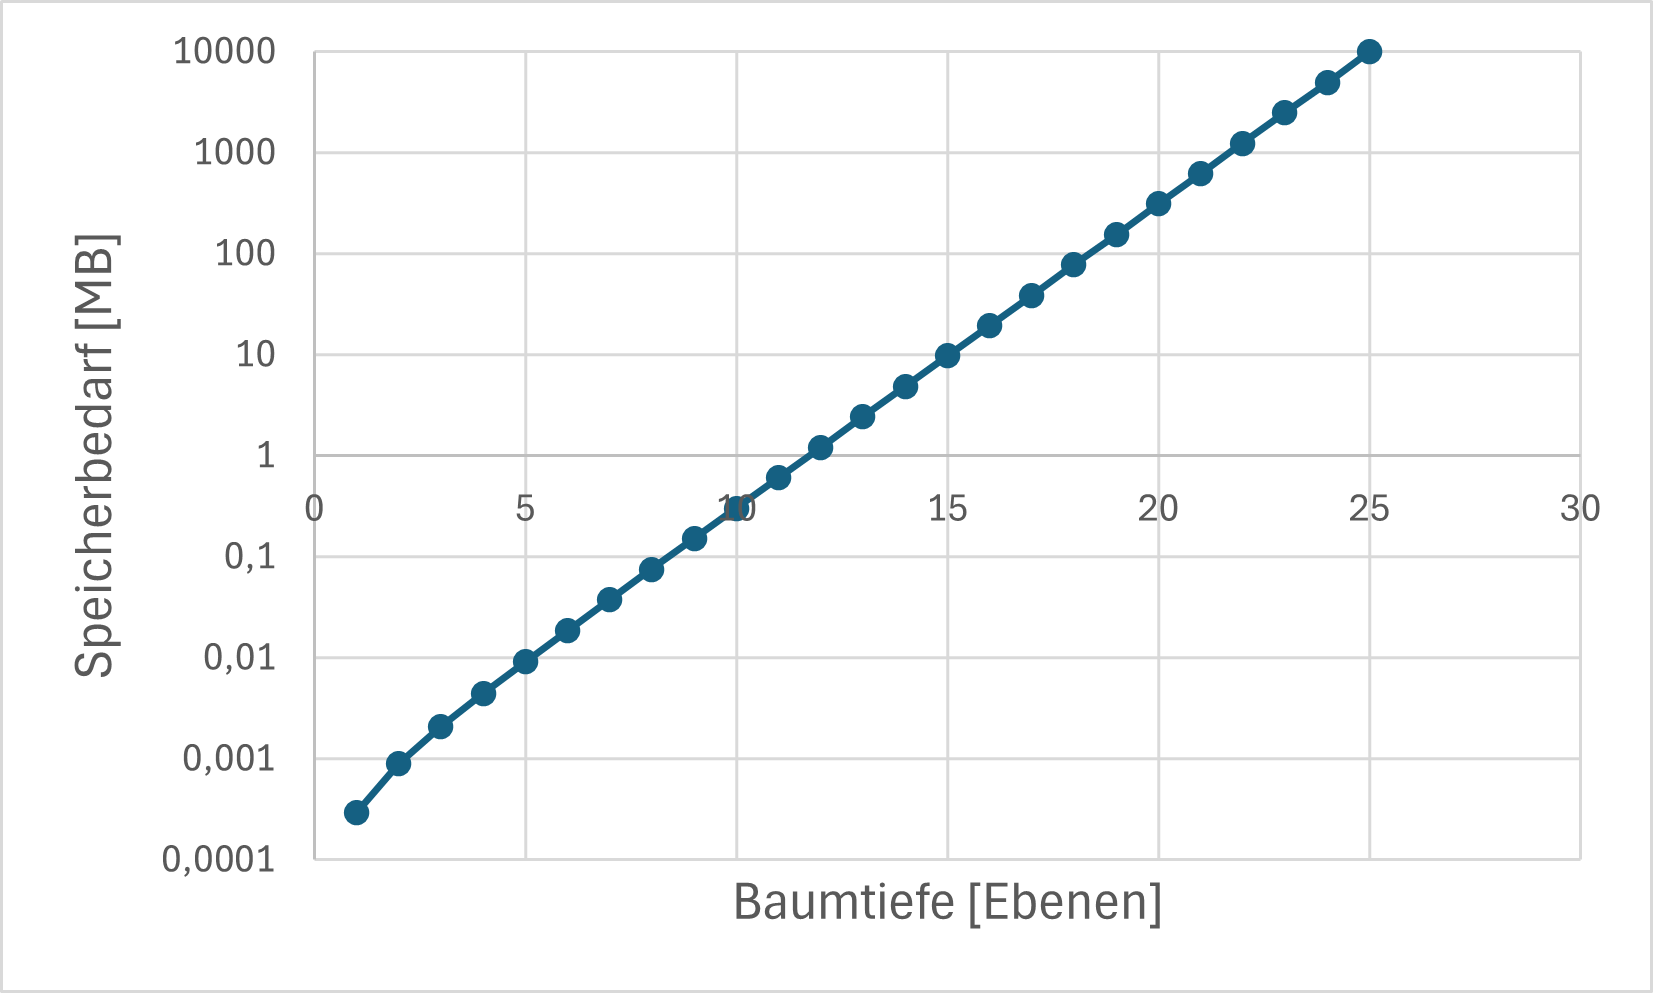
\includegraphics[width=\linewidth]{./diagrams/Speicherplatzbedarf.png}
    \captionof{figure}{Gesamtspeicherbedarf Quader in Megabyte}
\end{minipage}
\vspace{0.5cm}\\
Dementsprechend ist der ausschlaggebende Faktor für die maximale Baumtiefe nicht etwa die Schnelligkeit 
des Prozessors oder der GPU, sondern der im RAM verfügbare Speicherplatz. 

\newpage
\subsection{Einfluss der Speicherhierarchie}
\vspace{-0.25cm}
Da die Quader jeder Ebene in einem Array (bzw. Vector) gespeichert werden, sind ihre Daten in einem 
zusammenhängenden Bereich im Hauptspeicher abgelegt.\\
Bei OpenMP wird direkt über dieses Array iteriert, weshalb die Zugriffszeit auf die Daten durch Caching stark 
reduziert werden kann. Im Vergleich dazu wäre der Einsatz einer Verkettete Liste für die gleiche Aufgabe
deutlich langsamer.\\
Bei OpenCL müssen die Daten jedes Mal von der CPU auf die GPU und zurück übertragen werden. Dadurch spielt der Cache
hier eine untergeordnete Rolle. Allerdings müssen die Daten nichtsdestotrotz in einem zusammenhängenden Block abgelegt sein, 
weil für die Erzeugung der Buffer ein Zeiger auf den zu kopierenden Speicherbereich benötigt wird. Dies ermöglicht
vermutlich eine Art DMA über PCIe. Eine Beschleuningung des Programmanblaufs durch Caching ist im mit OpenCL parallelisierten
Bereich deshalb nur bei der Übertragung von Werten in den Renderer möglich. Diese erfolgt wiederum durch eine mit OpenMP
paralleliserte Schleife, die über einen zusammenhängenden Speicher (Vector) iteriert.

  